% ****** Start of file apssamp.tex ******
%
%   This file is part of the APS files in the REVTeX 4.1 distribution.
%   Version 4.1r of REVTeX, August 2010
%
%   Copyright (c) 2009, 2010 The American Physical Society.
%
%   See the REVTeX 4 README file for restrictions and more information.
%
% TeX'ing this file requires that you have AMS-LaTeX 2.0 installed
% as well as the rest of the prerequisites for REVTeX 4.1
%
% See the REVTeX 4 README file
% It also requires running BibTeX. The commands are as follows:
%
%  1)  latex apssamp.tex
%  2)  bibtex apssamp
%  3)  latex apssamp.tex
%  4)  latex apssamp.tex
%
\documentclass[reprint,
 amsmath,amssymb,nobibnotes,
 aps, floatfix]{revtex4-1}

\usepackage{graphicx}% Include figure files
\usepackage{dcolumn}% Align table columns on decimal point
\usepackage{bm}% bold math
\usepackage{url}
\usepackage{units}
\usepackage{physics}
\usepackage[table,xcdraw]{xcolor}
\usepackage[normalem]{ulem}
\useunder{\uline}{\ul}{}
\usepackage{adjustbox}
\usepackage{float}
\usepackage{lettrine}
\usepackage{lipsum}
\usepackage[%  
    colorlinks=false,
    pdfborder={0 0 0},
    linkcolor=blue
]{hyperref}
\usepackage{array}
\newcolumntype{P}[1]{>{\centering\arraybackslash}p{#1}}
\newcommand*{\balancecolsandclearpage}{%
  \close@column@grid
  \cleardoublepage
  \twocolumngrid
}
%\usepackage{hyperref}% add hypertext capabilities
%\usepackage[mathlines]{lineno}% Enable numbering of text and display math
%\linenumbers\relax % Commence numbering lines

%\usepackage[showframe,%Uncomment any one of the following lines to test
%%scale=0.7, marginratio={1:1, 2:3}, ignoreall,% default settings
%%text={7in,10in},centering,
%%margin=1.5in,
%%total={6.5in,8.75in}, top=1.2in, left=0.9in, includefoot,
%%height=10in,a5paper,hmargin={3cm,0.8in},
%]{geometry}

\begin{document}


\title{How the Pros Play: \\ An analysis of lichess.org's ranked chess games }% Force line breaks with \\
%\thanks{A footnote to the article title}%

\author{Alex Jose}
\author{Davis Trinh}
\author{Jing Duan}
\author{Joe Strawinski}
 %\altaffiliation[Also at ]{Physics Department, XYZ University.}%Lines break automatically or can be forced with \\
 %\email{Second.Author@institution.edu}
\affiliation{%
The Data Analytics Boot Camp at The University of North Carolina at Chapel Hill\\
 %This line break forced with \textbackslash\textbackslash
}%
\date{\today}% It is always \today, today,
             %  but any date may be explicitly specified
\begin{abstract}
\begin{center}
    \textbf{ABSTRACT}
\end{center}
Chess is the most popular board game in the world. It’s popularity continues to expand as it has become more accessible to play thanks to online services. Many of us have casually played a game of chess before (or at least heard of chess), but have never considered the consequences of the first move we take or the sophisticated strategies that have been developed by advanced players. Using chess match data obtained via Kaggle and Lichess, we answered several questions that had piqued our interest. From our results, we observed: the player who goes first has a slight statistical edge over the player who goes second, upsets are common however they occur much less frequently as the disparity in skill level widens, competitive matches often end in resignation rather than checkmate, matches tend to last longer when players are evenly matched, and that there are statistically favorable and unfavorable opening moves.
\end{abstract}

%\pacs{Valid PACS appear here}% PACS, the Physics and Astronomy
                             % Classification Scheme.
%\keywords{Suggested keywords}%Use showkeys class option if keyword
                              %display desired
\maketitle

%\tableofcontents

\section{\label{sec:level1}Introduction}
\lettrine{C}{hess} has never been more accessible to play. A large contribution towards the community's growth is it's expansion into online services. The top chess players in the world play online matches and stream themselves on sites such as YouTube and twitch.tv.  Lichess.org, a popular site for online chess games currently serves over 35 million ranked matches a month.

A single chess game  can be broken into three stages: Opening, Mid-game and End-game. The opening consists of the initial set of moves played by both white and black. Traditionally white makes the first move, and it is black's role to respond. The opening "sets the stage" of the game as well as the overall pace of the game. Since openings can be described in approximately 5 turns, it is a common point of study for high level chess players. Most openings in chess have been classified under the Encyclopedia of Chess Openings (or ECO). 

By Mid-Game and End-Game both players are now no longer relying on previously studied positions, and instead use their general intuition and skill to pick positions that will place their opponent in \textit{check}. 

Emulation is a large part of improving in chess. Studying great chess players and analyzing common positions is common practice for mid and high level players. In this report we obtain general statistics on the online player base, and attempt to extract characteristics of game play that distinguish highly rated players. We also demonstrate how online chess can be used to analyze and improve your own games through the use of player specific analysis. 

\section{\label{sec:level2}Data Acquisition and Cleaning}
Although Lichess.org hosts fewer games than its main competitor, chess.com, it has a more accessible API. Furthermore it is possible to download every ranked game that has ever been played on the site. For general usage statistics we use a Kaggle dataset that was obtained using API calls on 1500 ranked players. This set contains approximately 20,000 ranked games. The only cleaning required for this set was removing games that were not completed.

A CSV was also generated using the set of all ranked games of May, 2015. This set was contained in a PGN format, which was read using the python-chess module.

The sets include game type, which player won, and their opening moves. The entire PGN move list is recorded as well in a standard format. Both sets contain the Elo of both white and black. Elo is a numerical ranking system that is calculated using the relative skill of a player. A higher Elo player has better, and more frequent wins. The highest ranked players in the world have Elo ratings of 2800 

A wrapper for the Lichess API was used to collect all of the Lichess.org games played by chess grandmaster Zhigalko Sergei. This set contains the same information as the other sets we collected. For this set, we applied the python-chess module to parse the move list and create virtual boards. The string representing the board of was then manipulated to conform to a 2D array.

Games obtained from the raw PGNs that were missing relevant headers were removed from our analysis.
\section{\label{sec:level3}Results and Analysis}
\subsection{General Game Statistics}
Chess rules dictate that the player using the white pieces makes the first move. This results in a slight favor towards white. White wins 50\% of games while Black only wins 47\% of games.

We examined several relationships relating to the number of turns played in a game. It is worth noting that most games do not end with "check mate." Instead, most players resign a few turns before they inevitably lose (Figure \ref{fig:resign}.) 

\begin{figure}
    \centering
    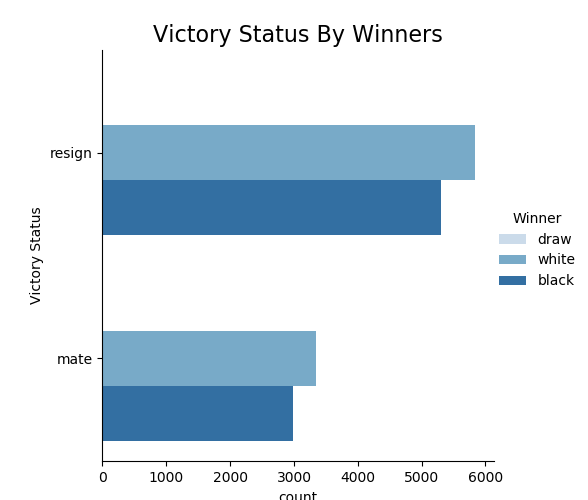
\includegraphics[scale=.5]{image1.png}
    \caption{The amount of winning games ending in resign or mate. This plot also shows that a majority of winning games are won by white.}
    \label{fig:resign}
\end{figure}

The number of turns for draws is significantly larger than turns for winning games. Intuitively this is because draws tend to occur when there are not enough pieces in play for either player to check mate their opponent. This results in a repetitive back and forth chase, that ends in a draw. In figure \ref{fig:draw} it can be seen that games that black wins take more turns on average. This could be a reflection of black's turn disadvantage.
\begin{figure}
    \centering
    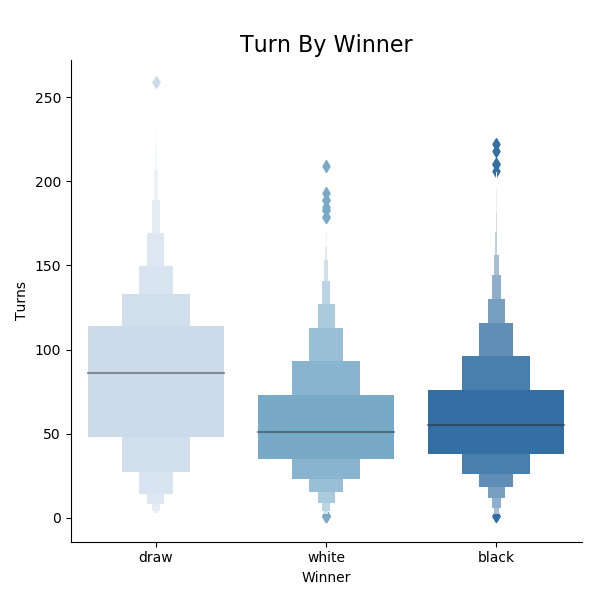
\includegraphics[scale=.5]{image5.png}
    \caption{A box and whisker plot with histogram and outliers.}
    \label{fig:draw}
\end{figure}

We analyzed the relationship between player's skill and the amount of turns in a game. Although it is not strongly correlated, when the average skill of both players is larger, games have more turns in general (Fig \ref{fig:elo_turn}. When there is a large skill differential between the players, there is a slight trend towards games ending with fewer turns (Figure \ref{fig:elo_diff_turn}). These trends agree with our expectations, yet we are surprised that the trends are not pronounced. 

\begin{figure}
    \centering
    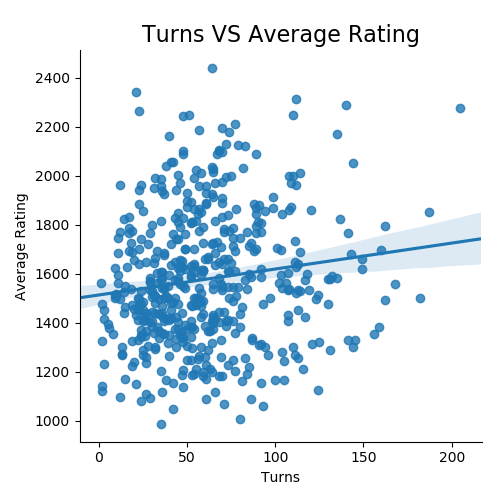
\includegraphics[scale=.5]{image4.png}
    \caption{Points represent individual games. Average rating is calculated as the average Elo between players.}
    \label{fig:elo_turn}
\end{figure}


\begin{figure}
    \centering
    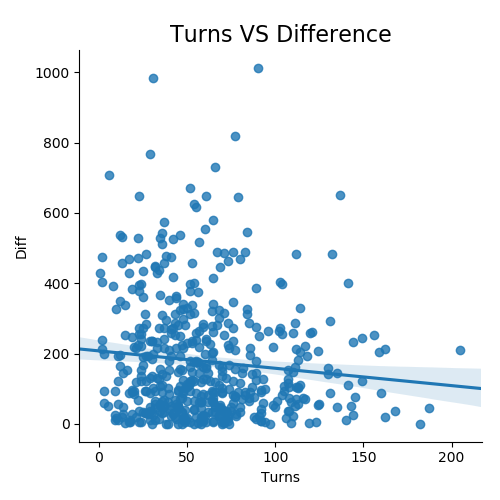
\includegraphics[scale=.5]{image6.png}
    \caption{The magnitude of the difference between Elo was used to approximate the skill gap. Within statistical uncertainty, games with a large skill gap end in fewer turns.}
    \label{fig:elo_diff_turn}
\end{figure}

On Lichess, it is possible for users to play games that do not contribute to their ranking. We checked if these unranked games had different features compared to ranked games. Based on figure \ref{fig:rated}, the distribution of games played is mostly the same between ranked and unranked games. The most significant difference is higher ranked players experience more draws when playing unranked games. This could be indicative of players opting for more experimental techniques and less of a drive to win. 

\begin{figure}
    \centering
    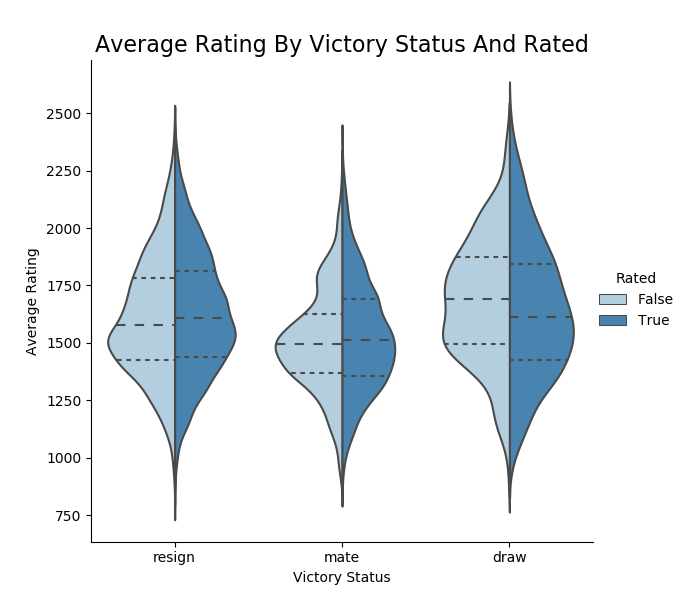
\includegraphics[scale=.5]{image8.png}
    \caption{A set of histograms of victory status corresponding to the average rating between players. It also shows the differences between ranked and unranked games.}
    \label{fig:rated}
\end{figure}
\subsection{Elo based trends and Upset Potential}

In our investigation we looked at a 2,000,000 game sample from Lichess.org and found that about one third of the total matches ended up in an upset - defined here as a draw or loss for the higher rated Elo player Figure \ref{fig:Base_Upset}. To further elaborate on this we looked at how often upsets occur when there is a wide Elo disparity between players.

\begin{figure}
    \centering
    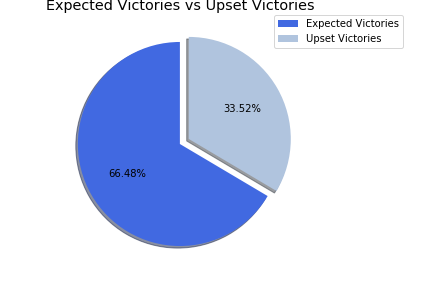
\includegraphics[scale=.5]{davis_image5.png}
    \caption{Overall Upset Potential}
    \label{fig:Base_Upset}
\end{figure}

As one would intuitively expect, the frequency of upsets decreases as the skill differential between two players increases. From figure \ref{fig:upset_elo}, we can see that the distribution of upsets is skewed to the left. A majority of upsets, by our definition, occurs when both players are evenly skilled (ΔElo < 500).  

\begin{figure}
    \centering
    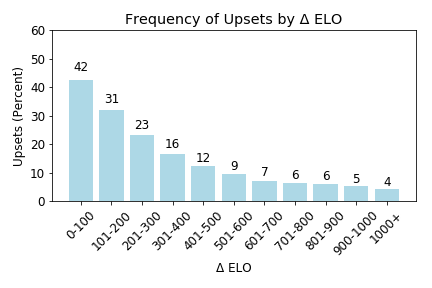
\includegraphics[scale=.5]{davis_image2.png}
    \caption{Upset Potential, Binned by Elo difference}
    \label{fig:upset_elo}
\end{figure}
As previously stated, white's first move advantage impacts white's overall win percentage (Figure \ref{fig:overall_wins}). Does white still hold a slight advantage over black as skill differential increase? According to the data (Table \ref{fig:Color_win_elo_gap}), white generally retains a slight edge over black across most Elo differential groups, however the edge appears to diminish when there’s a vast disparity in skill (ΔElo > 800).
\begin{figure}
    \centering
    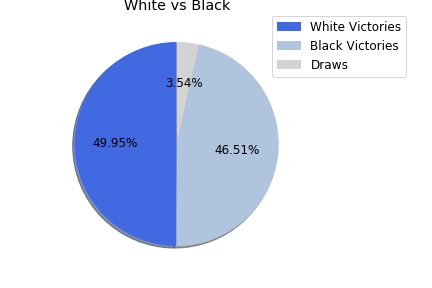
\includegraphics[scale=.5]{davis_image3.png}
    \caption{Overall win percentage based off of 2 million ranked games.}
    \label{fig:overall_wins}
\end{figure}
\begin{figure}
    \centering
    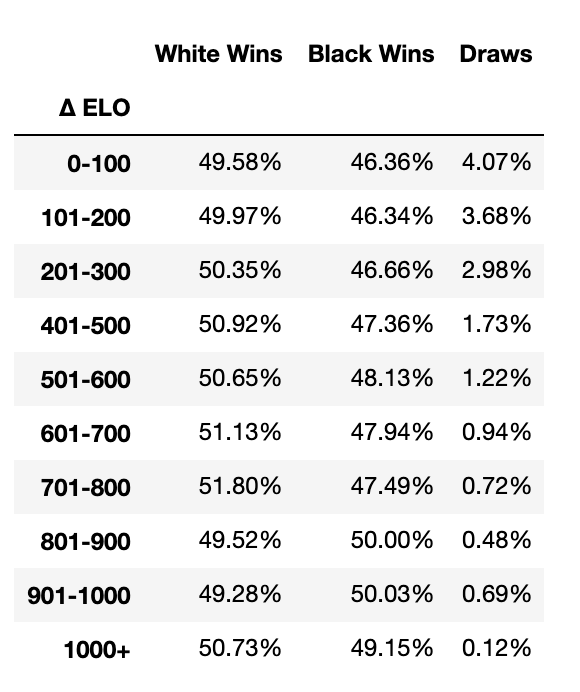
\includegraphics[scale=.5]{davis_image1.png}
    \caption{Win percentage for white and black, grouped by skill differential. White's first move advantage is less prominent when there is a large skill gap}
    \label{fig:Color_win_elo_gap}
\end{figure}
Does white still hold a slight advantage over black when black is favored? Analysis of the data suggests that in matches between evenly skilled player (ΔElo < 500), where the favored player went first, had a slightly higher win rate relative to when the favored player went second. Once again, this slight advantage diminishes as the gap between skill increases. Matches where ΔElo > 800 saw the advantage change slightly in favor of the player who went second (Figure \ref{fig:elo_bin_upset}).

\begin{figure}
    \centering
    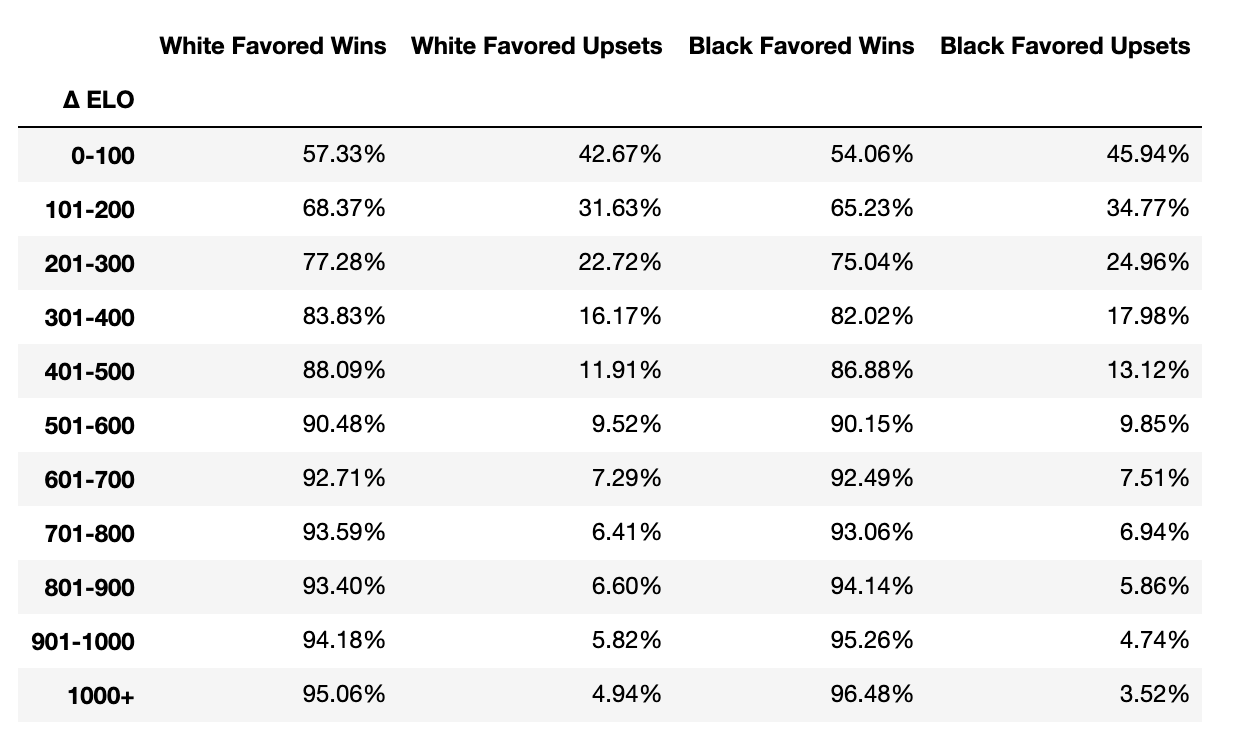
\includegraphics[scale=.4]{davis_image6.png}
    \caption{Percentage of wins based on which color player was favored. This statistic is analyzed for different bins of skill disparity.}
    \label{fig:elo_bin_upset}
\end{figure}

\subsection{Opening Move Analysis}
An important clarification to be made is that an opening consists of multiple moves. At what point an opening is classified as an opening is a relatively arbitrary decision. Some openings branch into variations and numbers. For this reason, when studying the effectiveness of a particular variation, we limit ourselves to only positions that occurred frequently. We calculate the "average score" of an opening by looking at white's success for individual games. An opening is awarded a single point if white wins, zero for a draw, and minus one for white's loss. These game scores were then averaged for groups of the the same opening. 
\subsubsection{Openings with Variation}
The table \ref{fig:white_open} summarizes the most successful openings with variation for white.
\begin{figure}[h!]
    \centering
    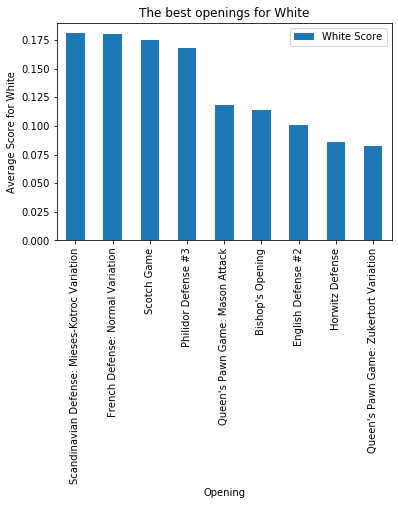
\includegraphics[scale=.5]{openings_white.png}
    \caption{The most successful openings positions for white.}
    \label{fig:white_open}
\end{figure}

The opening with the highest score for white is a the Mieses-Kotroc variation of the Scandinavian Defense. In this opening black takes white's pawn with his queen. While this gives an early piece advantage, it seems like it forces black to defend his queen early. This ultimately makes it one of the worst opening positions for black.

\begin{figure}[H]
    \centering
    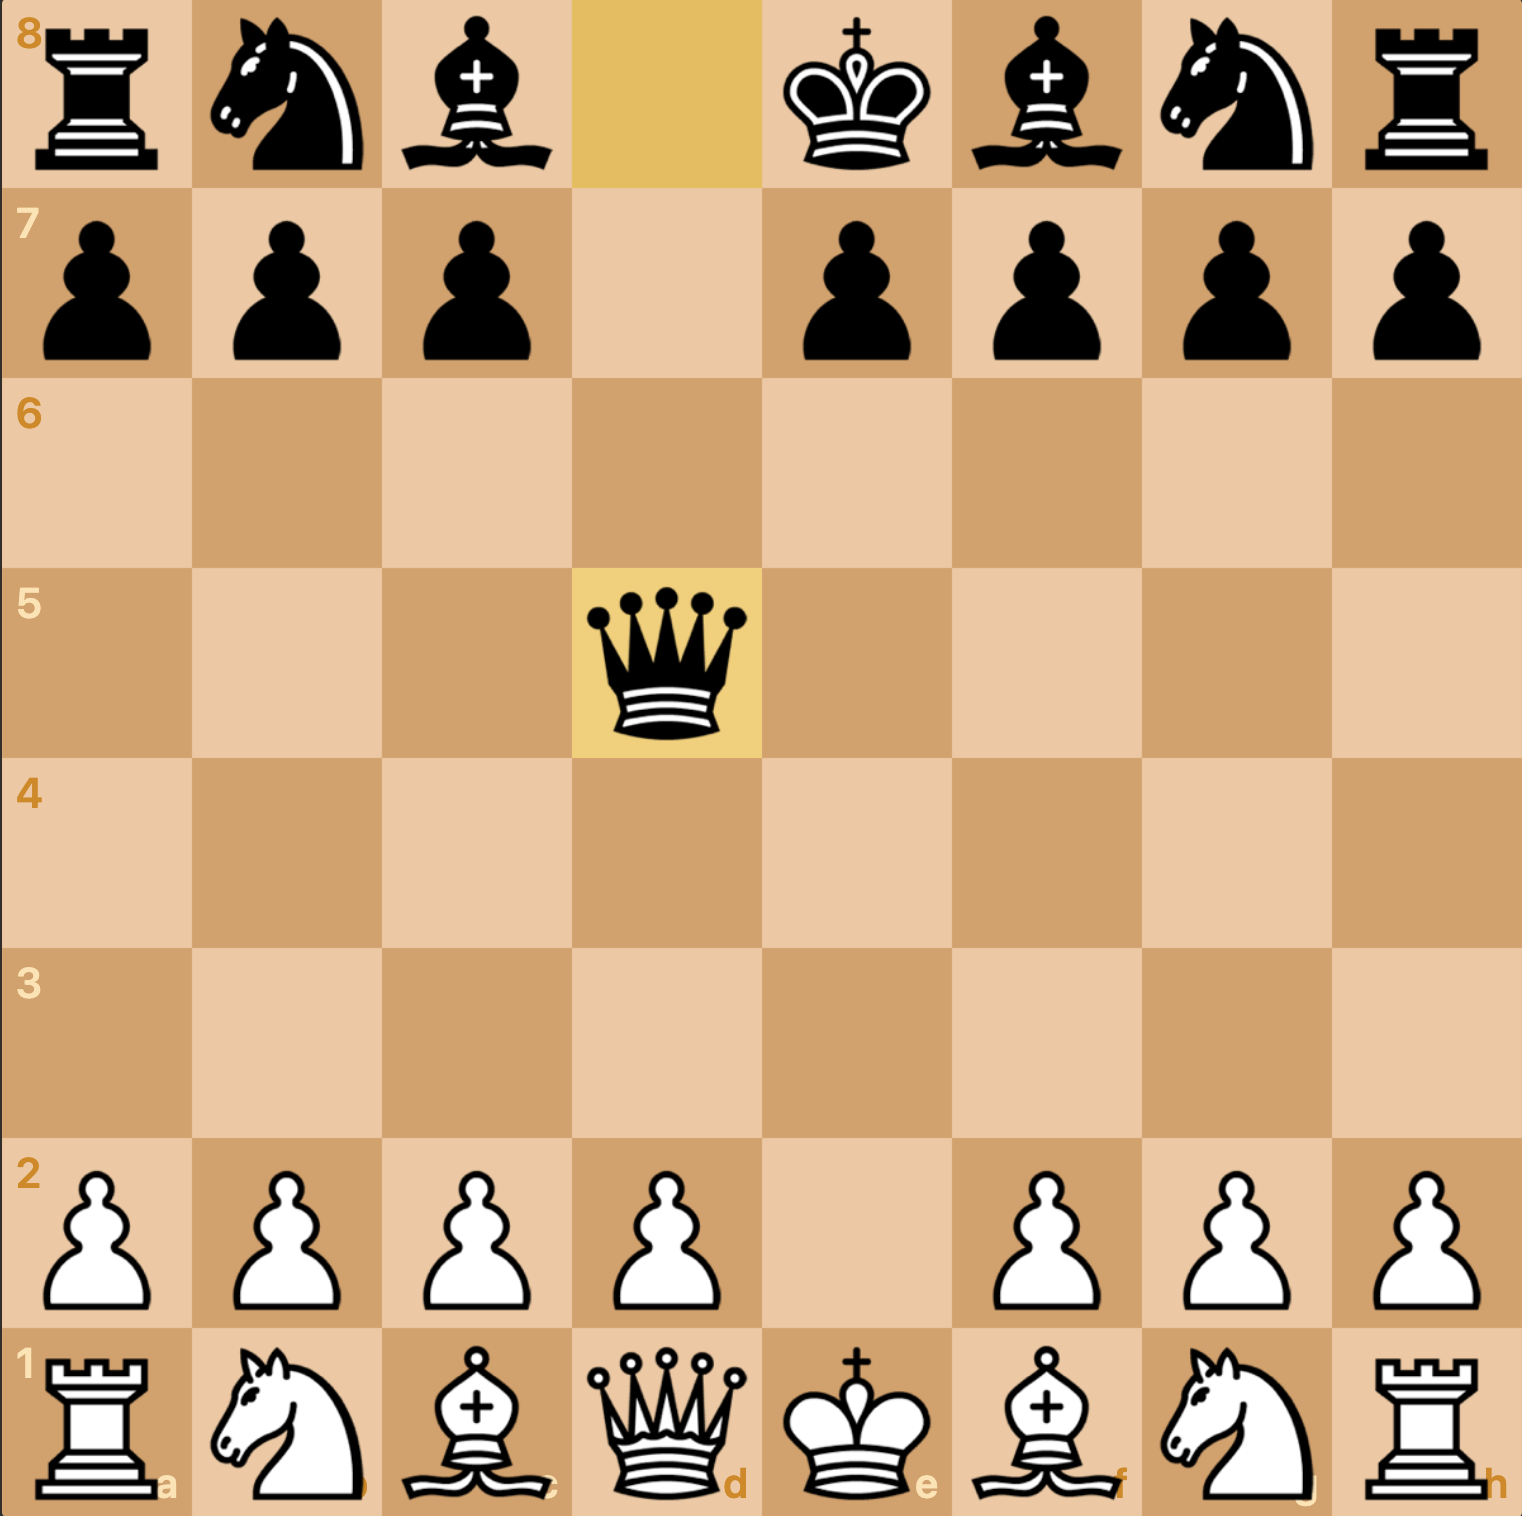
\includegraphics[scale=.20]{Mieses-Kotroc.png}
    \caption{The Scandanavian Defense: Mieses-Kotroc Variation}
    \label{fig:mieses}
\end{figure}

Figure \ref{fig:black_opening} contains the worst scoring openings for white.

\begin{figure}[h!]
    \centering
    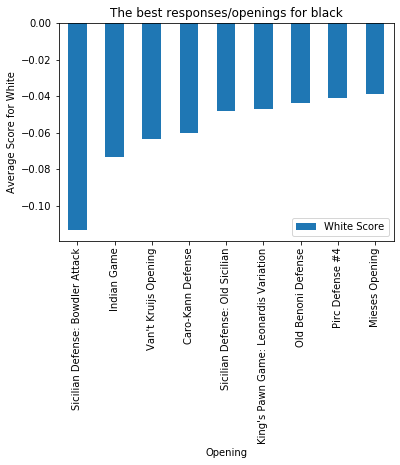
\includegraphics[scale=.5]{openings_black.png}
    \caption{The best opening positions for black}
    \label{fig:black_opening}
\end{figure}

The worst position for white is the Bowdler Attack variation on a Sicilian Defense. White opens up the pawn in front of his king. Black responds making room for the queen. Then white moves their bishop to half board. This is a popular, yet disadvantages position for white. White has exposed their king and bishop, while black has the opportunity to work with their queen.

\begin{figure}[H]
    \centering
    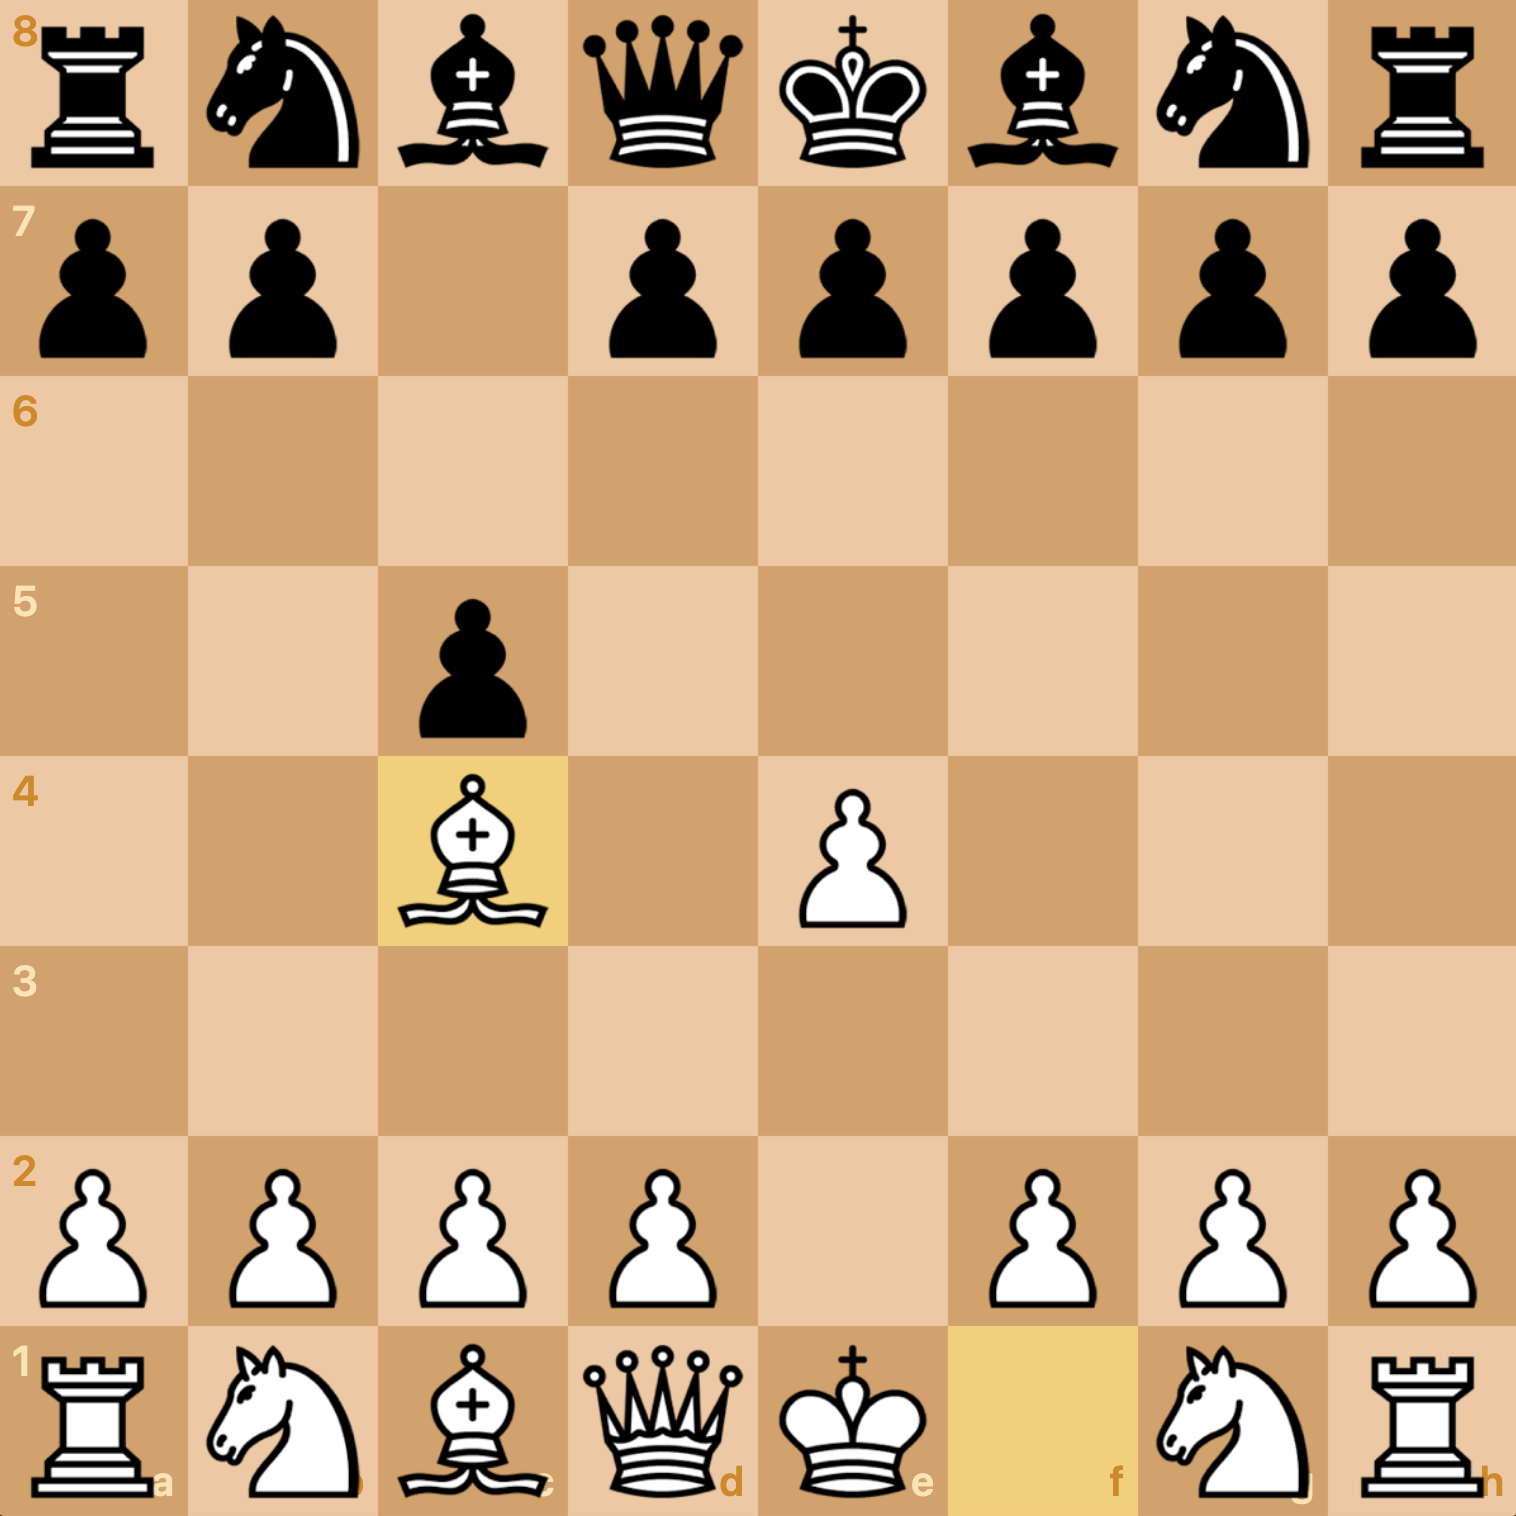
\includegraphics[scale=.2]{bowlderattack.png}
    \caption{Sicilian Defense Opening: Bowlder Attack Variation}
    \label{fig:Bowlder}
\end{figure}
\subsubsection{Opening Categories and success within Categories }
Taking a deeper look at the data, we analyzed game outcomes of variations (sub-category) in relation to the outcomes of the grouped opening (category).  Our comparison of the individual variations vs. the success of the overall group within the opening category, illustrates that not all variations are created equal.  It is worth noting that differences in game outcomes exist among variations and although a category of opening may indicate favorable or unfavorable success for either player based on the data, players should study and understand the differences in success for variations within an opening move in order to maximize their results.
To further our investigation, we judgmentally selected (based on popularity) two openings to analyze. The Queen’s Gambit and Ruy Lopez are two of the most widely touted opening moves for white.
The Queen’s Gambit includes four variations.  According to the lichess.org data, all variations produced favorable outcomes for white.  However, a sizable difference exists between the Queen’s Gambit (most favorable: 0.2908) and Queen’s Gambit Declined (least favorable 0.0934).  These outcomes are in-line with our expectation as the Queen’s Gambit Declined is a response from black declining White's temporary pawn sacrifice as a defense to the Queen’s Gambit 1.d4.
We also analyzed the Ruy Lopez, also referred to as the Spanish Opening.  Among highly rated players, the Ruy Lopez is often regarded as one of the best opening moves for white. Note, it was a favorite of Bobby Fisher and more than 100 variations exists for the opening that begins with white creating a potential pin of the d-pawn or Knight. The Ruy Lopez immediately sparks an attack, putting pressure on black.   However, due to the complexity and number of variations for the Ruy Lopez, a player should study and understand all the variations to maximize success. Our analysis focused on the top and bottom three variations.
The least favorable outcomes for white include:
-    Closed Variations: Lutikov Variation
-    Closed Variations: Worrall Attack
-    Open Variations: Karpov Gambit
The most favorable outcomes for white include:
-    Central Countergambit
-    Brentano Gambit
-    Retreat Variation
\subsection{Player Specific Analysis: GM|Zhigalko Sergei}
\begin{figure*}[hb]
    \centering
    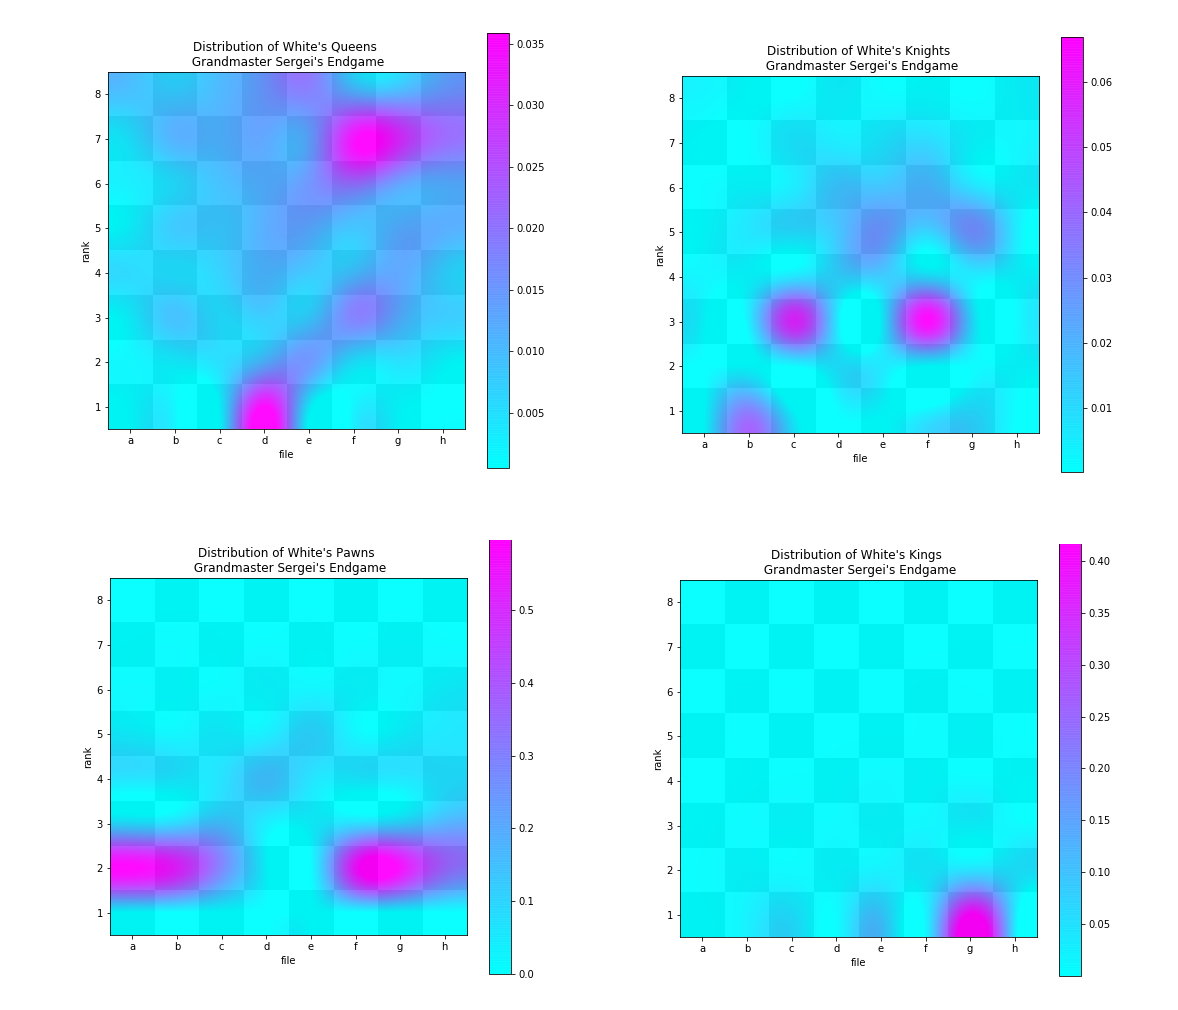
\includegraphics[scale=1.3]{heatmaps.png}
    \caption{Heatmaps of piece locations taken from winning board configurations.}
    \label{fig:my_label}
\end{figure*}

Sergei is ranked top 300 in the world by the World Chess Federation. His board game winning configurations were analyzed to provide insight towards top level end-game strategies. Heatmaps were generated from his winning games.

From the knights map we see that the GM favors to keep knights close the center of the board, slightly closer to his side. This position pressures a large range of squares, meanwhile protecting pieces closer to his side of the board.

Pawns on the outside tend to be developed less often. By moving the center pawns up the GM allows more key pieces to be developed: bishop, queen etc. An interesting trend here is the asymmetry. The right most pawn is moved more often than the left most pawn.

As expected, the king is often protected at the right corner of the board. It is worth noticing that the most frequent square is not the original starting square for the king. It is likely the king is moved to this square using a technique known as “castling”.

The queen tends to be placed in a few distinct patterns. The queen is found near the ends of the board, while also controlling the main center diagonals. His queen tends to take an extremely aggressive position on black's starting rows.


%\subsection{Work Functions?}
\cleardoublepage
\section{\label{sec:level5} Acknowledgements and Sources}
Opening boards were provided by chess.com. All data was sourced from lichess.org's API. Special thanks to cyanfish's python client for lichess's API.
\bibliography{sources}
\bibliographystyle{apsrev4-1}
\end{document}